\PassOptionsToPackage{hyphens}{url}
\documentclass[a4paper,fleqn]{cas-sc}
\usepackage{fontspec}
\usepackage{longtable,booktabs,array,calc,graphicx}
\providecommand{\tightlist}{\setlength{\itemsep}{0pt}\setlength{\parskip}{0pt}}
\renewcommand{\printorcid}{}  % anonymized: no author, so no empty "ORCID(s):" line
\newcounter{none}  % pandoc tables set \LTcaptype{none}; this longtable needs the counter
\def\tsc#1{\csdef{#1}{\textsc{\lowercase{#1}}\xspace}}
\begin{document}
\let\WriteBookmarks\relax
\def\floatpagepagefraction{1}
\def\textpagefraction{.001}
\shorttitle{nox-mem: a pre-specified comparison of agent memory systems}
\shortauthors{Anonymous}
\title[mode=title]{nox-mem: a single-file hybrid memory for LLM agents, and a pre-specified comparison against five memory systems}
\begin{abstract}
Persistent memory for large language model (LLM) agents is usually a service built from several databases and model calls. We describe nox-mem, a memory system that keeps each store in a single SQLite file, retrieves with BM25 and dense embeddings fused by Reciprocal Rank Fusion, and ranks with a hand-specified salience score whose changes pass a shadow phase before activation. Our main contribution is a comparison against five memory systems whose execution plan was committed to a public repository before the first run. On one corpus and query set (LoCoMo and LongMemEval, nDCG@10), the ordering depends on the configuration. Under each system's default embedder, Mem0 leads on LoCoMo (0.4686 vs 0.4263) and nox-mem on LongMemEval (0.5234 vs 0.4764), with 100 queries per dataset. With the embedder matched over all 2,482 queries, nox-mem leads Mem0 on both datasets and in all five represented query categories, with four residual confounds declared. EverOS, which requires a 4 B cross-encoder re-ranker, leads every system (overall 0.6455 against 0.5013 for nox-mem); Zep ranks third; Letta produced no number. Three findings cut against our own design: the severity signal (``pain'') in the salience score has no significant isolated effect (+0.0065, 95\% CI {[}−0.0143, +0.0338{]}, n = 31); section-aware ranking carries nearly all of the ablation gain; and on EverMemBench nox-mem trails MemOS on multi-hop questions (6.02\% vs 10.84\%) while leading it overall by 4.01 pp, both below the full-context baseline. The knowledge-graph path answers in 2.5 ms at the median, in one 399 MB process.
\end{abstract}
\begin{highlights}
\item A single-file SQLite memory for LLM agents, with BM25 and dense retrieval fused
\item Pre-specified comparison with five memory systems over 2,482 queries
\item The ordering of nox-mem and Mem0 flips when the embedder is matched
\item EverOS, which requires a 4B re-ranker, leads all systems on nDCG@10
\item The severity signal in the salience score shows no significant isolated effect
\end{highlights}
\begin{keywords}
LLM agents \sep agent memory \sep hybrid retrieval \sep reciprocal rank fusion \sep retrieval evaluation \sep reproducibility
\end{keywords}
\maketitle

\section{Introduction}

An LLM agent that runs for weeks loses what it learned whenever its context window is reset or compacted: decisions, incidents, who owns what. Memory systems for agents address this by writing what the agent should keep into an external store and retrieving from it on later turns. Several such systems are now available as libraries or services, among them Mem0 (Chhikara et al., 2025), Zep (Rasmussen et al., 2025), Letta, formerly MemGPT (Packer et al., 2023), and EverOS (Hu et al., 2026a). They differ in what they store (raw text, extracted facts, graphs), in how they rank, and in what they need to run: most combine a relational database, a vector database and one or more paid model APIs.

Two questions matter to someone choosing among them, and the published record answers neither well. The first is how the systems compare on retrieval quality when given the same corpus and the same queries. Vendor reports use different benchmarks, different metrics (often an LLM-judged answer accuracy, not a retrieval metric) and different backbones, and the benchmark a vendor reports on is sometimes authored by the vendor (Hu et al., 2026b). The second is what a memory system costs to operate: how many services, which keys, how much memory, how long each query takes.

This paper reports a system built for the second question and a comparison designed for the first. nox-mem stores each agent's memory in one SQLite file. Retrieval combines a lexical channel (SQLite FTS5 with BM25; Robertson \& Zaragoza, 2009) and a dense channel (one embedding model, exact search through sqlite-vec; Garcia, 2024), fused by Reciprocal Rank Fusion (RRF; Cormack et al., 2009). Ranking adds a salience score built from hand-set weights over importance, recency, access and an operator-assignable severity we call \emph{pain}, and every change to the ranking runs first in a shadow mode that logs without reordering. Nothing in the loop is learned. The system has served a fleet of six agents in production since March 2026.

The comparison is pre-specified: its execution plan, principles and anti-cherry-pick rules were committed to the public repository before the first run, though not registered with an external registry. It covers five competing systems (Mem0, Zep, Letta, agentmemory (2026) and EverOS) on one corpus of 6,822 documents drawn from LoCoMo (Maharana et al., 2024) and LongMemEval (Wu et al., 2025), scored by nDCG@10 against fixed gold labels.

Our contributions are:

\begin{enumerate}
\def\labelenumi{\arabic{enumi}.}
\tightlist
\item
  \textbf{A pre-specified, same-corpus retrieval comparison} of six memory systems (Section 4), reported under each system's native embedder and under a matched embedder, with every unfavourable result and every deployment failure reported beside the favourable ones. The ordering of the top two systems reverses between the two settings; a third system, with a mandatory 4 B cross-encoder, leads both.
\item
  \textbf{A description of a single-file memory design} (Section 3) whose retrieval runs at 2.5 ms median on its knowledge-graph path and 529 ms on its hybrid path, in one process with a 399 MB resident set, and needs no third-party key when embeddings are switched off.
\item
  \textbf{An ablation and a cross-benchmark evaluation} (Section 5) that locate where the ranking gains come from. They come from section-aware ranking over structured entity files, not from the severity signal the system was first built around.
\end{enumerate}

Three results run against the system's own framing, and we report them in the abstract for that reason. The severity signal has no significant isolated effect on retrieval. Section-aware ranking, a simpler mechanism, carries the ablation gain. And on the multi-hop track of EverMemBench, nox-mem trails the best published memory system on the same backbone. We do not claim state-of-the-art results: EverOS outperforms nox-mem on both datasets of the comparison, and on EverMemBench the full-context baseline outperforms both memory systems we compare.

The rest of the paper is organized as follows. Section 2 places the design and the comparison in the literature. Section 3 describes the system. Section 4 reports the cross-system comparison. Section 5 reports the ablation, the EverMemBench and LongMemEval evaluations and the operational profile. Section 6 discusses what the results support and their limits, and Section 7 concludes.

\section{Related work}

\subsection{Memory systems for LLM agents}

Surveys organize agent memory by what is stored and how it is written, read and managed (Zhang et al., 2025a), and self-evolving agents by what, when, how and where they adapt (Gao et al., 2026). Against either taxonomy nox-mem is a narrow instance: one storage substrate, one embedding model, a hand-specified write and retention policy, and no learned component.

Deployed systems and their close relatives fall into several families. Vector stores with a metadata layer, such as Mem0 (Chhikara et al., 2025), extract facts from dialogue with an LLM and index them. Operating-system-style architectures, such as MemGPT (Packer et al., 2023), page items between a fixed context and archival storage; nox-mem does not page, and an item it fails to surface is ranked low rather than evicted, which a change to the ranker can recover. Temporal and graph services, such as Zep (Rasmussen et al., 2025), build a knowledge graph with validity intervals over the conversation. Memory operating systems, such as EverMemOS (Hu et al., 2026a) and MemOS (Li et al., 2025), organize memory into managed units with their own lifecycle; EverMemOS also re-ranks retrieved episodes with a re-ranker model, which the EverOS release we ran requires (Section 4.2). Graph-based retrieval for RAG, such as HippoRAG (Gutiérrez et al., 2024), HippoRAG 2 (Gutiérrez et al., 2025) and LightRAG (Guo et al., 2025), spends an LLM call per chunk to build the graph; nox-mem's graph path is a SQL and regular-expression walk over extracted relations with no LLM call at query time, which is why it is cheap and why it is less expressive on multi-hop questions. At the other end, MeMo (Quek et al., 2026) encodes new knowledge into a separately trained memory model, the opposite of an inspectable store.

\subsection{Scoring and forgetting}

The closest prior art to the salience score is Generative Agents (Park et al., 2023), which ranks a memory stream by recency, importance and relevance. We do not claim that shape as new. Two things differ. nox-mem adds a severity value persisted on each chunk and set by the operator or, by default, by a fixed keyword rule at ingest; and changes to the ranking layer pass a shadow phase before they reorder anything. MemoryBank (Zhong et al., 2023) forgets on an Ebbinghaus-style curve per item; nox-mem uses an integer retention window per chunk type, coarser but readable and editable in place.

A recent line of work learns the memory policy instead of fixing it: what to write (Mem-α; Wang et al., 2025), which management operation to apply (Memory-R1; Yan et al., 2025), when to curate context (Memory as Action; Zhang et al., 2025b), and how to keep a constant-size state across turns (MEM1; Zhou et al., 2025; MemAgent, Yu et al., 2026). Each replaces a hand-written rule with a trained one and reports gains from doing so. nox-mem takes the opposite position: a policy that fits on one screen, can be diffed and reverted, and cannot discover per corpus what a trained policy finds. This paper does not measure that gap.

\subsection{Raw history against constructed memory}

Most deployed memory systems construct something from the conversation before they retrieve: extracted facts, summaries, graphs. A group of controlled studies from 2026 asks whether that construction pays for itself, and mostly finds that it does not. Zhou et al.~(2026a) compared six explicit memory systems with retrieval over the raw history and found localized gains but no consistent advantage over a strong raw-history baseline. Their reproduction of LightMem (Fang et al., 2025) found that changing only the retriever over a fixed constructed store moved answer accuracy substantially, and that retrieval over constructed memory did not consistently beat retrieval over raw turns (Zhou et al., 2026b). Bao et al.~(2026) ranked naive retrieval with re-ranking over raw turns first among the compared memory systems, EverMemOS, MemOS and Mem0 among them, in most of their benchmark and model settings; He et al.~(2026) reached the same direction on a partly overlapping set of systems and different benchmarks. Yuan et al.~(2026) crossed three write strategies (raw chunks, extracted facts, summaries) with three retrieval methods and found retrieval to matter more than write-time sophistication. In a pre-registered test, Sharma and Lall (2026) found raw turns selected by a typed decision model non-inferior to an LLM-extraction memory at a tight context budget on LoCoMo, while extraction was more accurate at generous budgets. Constructed-memory systems continue to report strong results on the same benchmarks (Ma et al., 2025, among others: SimpleMem, Liu et al., 2026; RecMem, Dai et al., 2026; TiMem, Li et al., 2026).

nox-mem sits on the raw side of this divide: it retrieves stored passages verbatim, and its only construction step, the nightly extraction into topic files (Section 3.2), adds passages without replacing their sources. The finding of Yuan et al.~(2026) that the retrieval method dominates also anticipates ours, from a different direction: in Section 4 the embedder alone was enough to reorder two systems.

\subsection{Comparing memory systems}

Retrieval evaluation across heterogeneous collections follows the zero-shot discipline of BEIR (Thakur et al., 2021), and embedding evaluation the conventions of MTEB (Muennighoff et al., 2023). Both bear on a comparison of memory systems, because each system ships with its own embedder: a comparison under native defaults measures the system and its embedder together, and only a matched-embedder variant separates them, and then only partly (Section 4.5). Conversational memory benchmarks follow the multi-session setting of Xu et al.~(2022). LoCoMo (Maharana et al., 2024) and LongMemEval (Wu et al., 2025) provide gold evidence per question, which allows a retrieval metric; EverMemBench (Hu et al., 2026b) targets multi-party, long-horizon collaboration and reports accuracy per category, LLM-judged for open-ended recall and multiple-choice for memory awareness and profile understanding. HaluMem (Chen et al., 2025) measures hallucination in memory systems, a dimension we do not evaluate.

Studies that place several memory systems under one protocol are recent. MemoryAgentBench (Hu et al., 2026c) defines four competencies and finds that no method masters all of them; Wu et al.~(2026) re-implement existing methods as modules of one framework; Shao et al.~(2026) show that reliability loss with scale is not a single phenomenon. The raw-history studies above also compare systems under one harness, on answer accuracy. We found no study that compares Mem0, Zep, EverOS and Letta on a retrieval metric over one corpus, under both native and matched embedders, and with the deployment failures reported; that is the gap Section 4 fills.

\section{System}

\subsection{Storage}

Each store is one SQLite file in write-ahead-logging mode: one per agent plus a shared workspace store, opened by the same binary according to an environment variable. A store holds four kinds of table.

\begin{itemize}
\tightlist
\item
  \textbf{Chunks.} One row per passage, with its source file, type, dates, a severity (\texttt{pain}), a retention window (\texttt{retention\_days}), a section label for entity files (\texttt{section}, \texttt{section\_boost}), importance, access count and last access time. Provenance is per chunk: every search result carries the chunk identifier and its source file.
\item
  \textbf{Lexical index.} An FTS5 virtual table over the chunk text, kept in sync by triggers, with the \texttt{unicode61\ remove\_diacritics\ 2} tokenizer (accent folding, no stemming; it replaced a Porter stemmer that mis-stemmed Portuguese).
\item
  \textbf{Vector index.} A sqlite-vec virtual table of 3072-dimensional float32 embeddings from \texttt{gemini-embedding-001} (Lee et al., 2025), with a map table from vector row identifiers to chunk identifiers. Search is exact; there is no approximate index.
\item
  \textbf{Knowledge graph.} Entities and typed relations extracted by an LLM, each relation with a confidence that decays over time, a 90-day expiry unless reconfirmed, and a link to its evidence chunk.
\end{itemize}

An append-only audit table records destructive operations, and those operations take an atomic snapshot of the file before they run. In production on 2026-09-09 the main store held 67,724 chunks, and the seven stores together held 79,220.

\subsection{Ingestion and retention}

A file watcher (\texttt{inotifywait}) re-ingests a Markdown or text file 2 seconds after its last write. Ingestion splits Markdown on second- and third-level headings, sub-splits sections longer than 500 words, merges fragments shorter than 20 words into the previous chunk, and replaces all chunks of the file in one transaction, so re-ingestion is idempotent. The type of a chunk follows from the path of its file (decisions, lessons, people, projects, pending items, daily notes, shared team documents and so on), and the type sets its retention window: never for feedback and people, 365 days for decisions and projects, 180 for lessons, 120 for team documents, 90 for daily notes and for untyped chunks, 30 for pending items. Entity files have a fixed three-section shape (frontmatter, a compiled summary, a timeline) and are ingested section by section, so each chunk carries its section label.

A nightly job sends recent daily notes to an LLM, which extracts decisions, lessons and similar items into topic files; the watcher then re-ingests them. A \texttt{crystallize} command stores a caller-supplied procedure as one chunk, with no LLM involved. Duplicates are suppressed before they are appended (cosine similarity above 0.85, or word overlap above 70\% without embeddings) and logged.

\subsection{Retrieval}

Retrieval runs in three layers (Fig. 1).

\textbf{Lexical.} FTS5 scores the query with BM25 over the chunk text, source path and type, weighted 1.0, 0.5 and 0.5. The query sanitizer replaces every character that is not a letter, digit or space with a space.

\textbf{Dense.} The query is embedded with the retrieval-query task type (chunks use the retrieval-document type), and the nearest chunks are found by exact L2 search.

\textbf{Fusion.} The two ranked lists are merged by RRF with the standard constant k = 60 (Cormack et al., 2009); a chunk found by both is marked hybrid, and near-duplicates are removed by their first 50 characters.

Before fusion, each layer adjusts its scores with boosts that are summed, never multiplied by each other: \(\mathit{score} = \mathit{base} \times (1 + \sum \delta)\). A boost with weight w contributes δ = w − 1. Entity-file sections are weighted 2.0 (compiled), 1.5 (frontmatter) and 0.8 (timeline), with 1.0 for chunks without a section. Chunks of the decision, lesson, person, project and pending types receive δ = +1.0 in the lexical layer and +0.5 in the dense layer; chunks from the last 7 days receive +0.5 and +0.2. The salience term of Section 3.4 enters as one more delta, bounded to {[}−0.5, +0.5{]}. These deltas replaced earlier multiplicative boosts.

A separate \textbf{knowledge-graph path} answers entity queries by walking \texttt{kg\_relations} with SQL and regular expressions. It makes no model call at query time.

\begin{figure}[t]
\centering
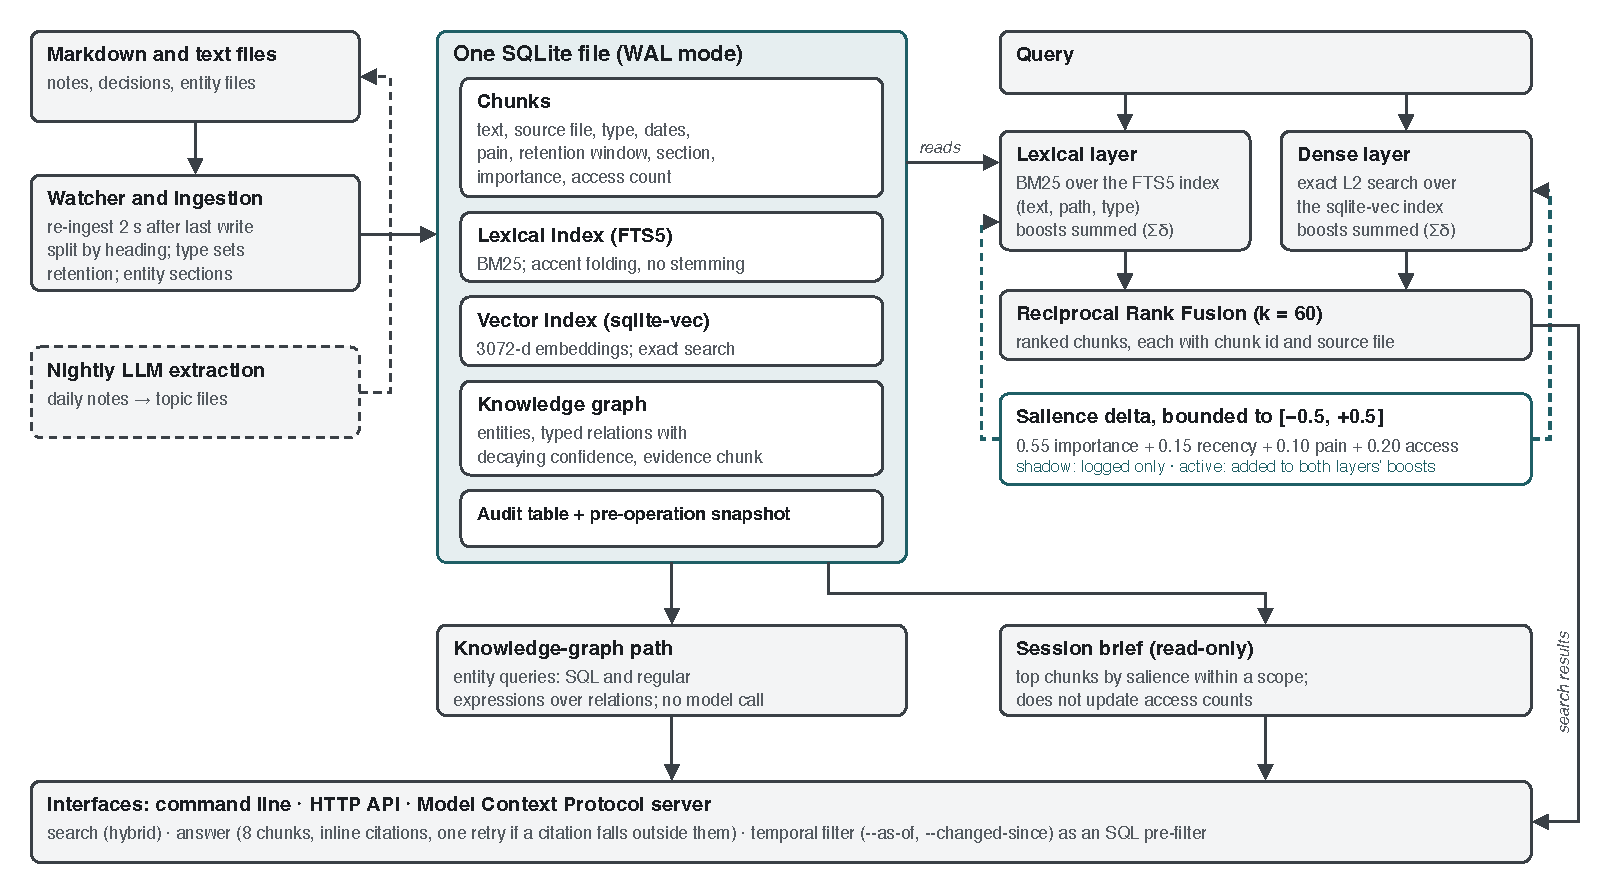
\includegraphics[width=\textwidth]{../figures/figure1.pdf}
\caption{Architecture of nox-mem: watcher and ingestion into a single SQLite file holding the chunk table, the FTS5 index, the sqlite-vec index and the knowledge graph; three retrieval layers (BM25, dense, RRF) with summed boosts and the salience delta; the knowledge-graph path; and the read-only session brief.}\label{fig1}
\end{figure}

\subsection{Salience and the shadow gate}

The salience score states a principle and ships in a different form. The principle is multiplicative: a memory should score high when it is recent, severe and important at once. In production it is additive,

\[\mathit{salience} = 0.55\,\mathit{importance} + 0.15\,\mathit{recency} + 0.10\,\mathit{pain} + 0.20\,\mathit{access},\]

because the product compressed 99.7\% of chunks into the range {[}0.05, 0.40{]} (Section 5.1). Importance follows the chunk type. Recency decays over the chunk's retention window and is recomputed at every retrieval from the time of last access, so no batch job ages the store and each access resets a chunk's clock. Pain is a severity in {[}0.1, 1.0{]} that the operator can set; otherwise a fixed rule assigns it at ingest, from a base per chunk type (0.2 when the type has none) raised by 0.5 when the text matches an incident or outage pattern. Nothing changes pain after ingest, so it measures whether a chunk talks about a failure, not how severe a failure was.

An environment variable sets the score's mode: \texttt{shadow} computes and logs the score without applying it; \texttt{active} adds salience − 0.5 to each layer's boosts; \texttt{off} disables it for ablations. Ranking changes are required to run in shadow mode before activation, with the score's distribution exposed on a health endpoint. Promotion from shadow to active is an operator decision.

\subsection{Session brief}

Each new session can load a brief: the top chunks by salience within a scope, returned by one HTTP call and injected at session start. The brief reads the store without touching access counts, so serving it does not feed the salience signal it ranks by. In production the first version served only 83 distinct chunks across 46.8k serves in 7 days (0.18\% diversity) while 931 recent, relevant chunks were never served; after two designs that failed in production, a diversity term that ranks by time since last serve reached all 184 eligible entity files on 2026-06-27. The measured account is in the supplementary material (S1, Section 3.5).

\subsection{Interfaces}

The same store is reached through a command-line interface, an HTTP API and a Model Context Protocol server. Three primitives form the public contract: hybrid \texttt{search}; \texttt{answer}, which retrieves 8 chunks by default, asks an LLM for an answer with inline chunk citations and retries once if a citation points outside the retrieved set; and a temporal filter (\texttt{-\/-as-of}, \texttt{-\/-changed-since}) applied as a SQL pre-filter on the candidates rather than as a ranking boost.

\section{Pre-specified comparison with five memory systems}

\subsection{Design}

The execution plan for the comparison was first committed to the public repository on 2026-05-21, before the first run (a capped smoke on 2026-05-23). It fixed six principles and an anti-cherry-pick statement. The principles: an identical corpus, ingested through each system's native API; an identical query set and gold labels; each system at its publicly documented default configuration; a cutoff of k = 10 for all; each system's native embedding provider, with an all-Gemini embedding-matched variant planned as a side experiment; and hardware declared per run. The anti-cherry-pick statement requires that both datasets and all query categories be reported whether favourable or not, and that a system that fails setup be reported with its reason rather than omitted. The plan named version ranges rather than exact pins, and it was not registered with an external registry. The tables in this section were written after the runs; where a run could not meet a principle, the text says so.

The plan also set a success criterion: nox-mem among the top three on at least two of four metrics (nDCG@10, R@10, MRR, latency). In the canonical run only three systems produced numbers, so the criterion holds by construction on the three quality metrics and carries no evidential weight, and latency was not captured across systems. We therefore do not report the criterion as passed and rest the comparison on the results below.

\subsection{Systems}

The five competitors were chosen by GitHub stars, recent commit activity and overlap with the scope of nox-mem (Table 3).

\textbf{Table 3.} Systems compared, with the versions recorded for each run and their default configurations.

{\def\LTcaptype{none} % do not increment counter
\begin{longtable}{@{}
  >{\raggedright\arraybackslash}p{(\linewidth - 6\tabcolsep) * \real{0.2500}}
  >{\raggedright\arraybackslash}p{(\linewidth - 6\tabcolsep) * \real{0.2500}}
  >{\raggedright\arraybackslash}p{(\linewidth - 6\tabcolsep) * \real{0.2500}}
  >{\raggedright\arraybackslash}p{(\linewidth - 6\tabcolsep) * \real{0.2500}}@{}}
\toprule\noalign{}
\begin{minipage}[b]{\linewidth}\raggedright
System
\end{minipage} & \begin{minipage}[b]{\linewidth}\raggedright
Install
\end{minipage} & \begin{minipage}[b]{\linewidth}\raggedright
Version
\end{minipage} & \begin{minipage}[b]{\linewidth}\raggedright
Default configuration
\end{minipage} \\
\midrule\noalign{}
\endhead
\bottomrule\noalign{}
\endlastfoot
nox-mem & npm & as of each run & FTS5 + \texttt{gemini-embedding-001} 3072-d + RRF, no cross-encoder \\
Mem0 & \texttt{pip\ install\ mem0ai} & \texttt{0.1.114} (canonical); 2.0.10 (embedding-matched run, Section 4.5) & OpenAI \texttt{text-embedding-3-small} 1536-d + faiss \\
Zep & Docker (Zep + Postgres) & \texttt{0.27.2} & \texttt{text-embedding-3-small} 1536-d, no re-ranker \\
Letta & \texttt{pip\ install\ letta} & \texttt{0.6.6} & SQLite backend; retrieval through an agent turn \\
agentmemory & daemon (REST) & as of 2026-06-15 & union store with namespace filter \\
EverOS & \texttt{pip\ install\ everos} & \texttt{1.3.1} & \texttt{gemini-embedding-001} 3072-d + \texttt{Qwen3-Reranker-4B} (mandatory) \\
\end{longtable}
}

\subsection{Corpus, queries and metric}

The corpus is the union of the LoCoMo and LongMemEval evidence passages, 6,830 documents carrying 6,822 distinct identifiers (eight pairs of different texts share an identifier; Section 4.5 explains how each system handled them). The query set holds 2,482 questions, 1,982 from LoCoMo and 500 from LongMemEval, each with gold evidence identifiers. Every gold chunk exists in the corpus. Retrieval is scored by nDCG@10 with binary relevance, with recall@10 and MRR alongside; a retrieved identifier counts once, at the rank of its first occurrence. Latency is wall-clock time around the adapter call.

Four runs produced the numbers reported here:

\begin{itemize}
\tightlist
\item
  the \textbf{canonical run} (2026-06-15), on a dedicated cloud pod, 100 queries per dataset, native embedders;
\item
  the \textbf{embedding-matched run} (2026-06-29), nox-mem and Mem0 both on \texttt{gemini-embedding-001} at 3072 dimensions, all 2,482 queries;
\item
  the \textbf{EverOS and Zep runs} (2026-09-10), all 2,482 queries, on a later host with a working Docker daemon.
\end{itemize}

\subsection{Native embedders: a split result}

In the canonical run, two of the five competitors produced quality numbers (Table 4). The three others were documented non-runs of that environment. Zep needs a Docker daemon, which could not start on the unprivileged pod (the kernel denied the network and namespace operations Docker requires); it ran later on a different host (Section 4.6). Letta installed and ran, but it routes retrieval through a full agent turn at about 16 minutes per query, so 100 queries per dataset would have taken days. EverOS then ran only as an HTTP service requiring two third-party credentials the run did not have; a later release removed that requirement (Section 4.6).

\textbf{Table 4.} Canonical run, native embedders, 100 queries per dataset, k = 10.

{\def\LTcaptype{none} % do not increment counter
\begin{longtable}{@{}llrrr@{}}
\toprule\noalign{}
Dataset & System & nDCG@10 & R@10 & MRR \\
\midrule\noalign{}
\endhead
\bottomrule\noalign{}
\endlastfoot
LongMemEval & \textbf{nox-mem} & \textbf{0.5234} & 0.6535 & \textbf{0.5494} \\
& Mem0 & 0.4764 & 0.6372 & 0.5107 \\
& agentmemory & 0.2803 & n/c & n/c \\
LoCoMo & \textbf{Mem0} & \textbf{0.4686} & 0.6171 & 0.4656 \\
& nox-mem & 0.4263 & 0.5504 & 0.4464 \\
& agentmemory & 0.1587 & n/c & n/c \\
\end{longtable}
}

n/c: not captured in this run.

Each of the two leading systems wins one dataset: nox-mem LongMemEval (+0.047 nDCG@10) and Mem0 LoCoMo (+0.042). agentmemory is a distant third on both. Because nox-mem and agentmemory were queried from a union store holding both datasets, an early reading was inflated by cross-dataset distractors (14.6\% of nox-mem's raw top-10 were off-dataset chunks). The canonical numbers therefore re-query at k = 30 and keep the top 10 within the active dataset. This raised nox-mem's LoCoMo score from 0.4173 to 0.4263, and Mem0 still wins LoCoMo.

Three differences in composition are declared rather than corrected. The embedders differ (Gemini 3072-d, OpenAI 1536-d), which is the point of the native-default stance. Mem0 used single-namespace stores while the other two used the filtered union store. And Mem0's LoCoMo store lost about 5\% of its vectors at ingest, to a thread leak in its default telemetry (Section 4.8). The per-query outputs of this run were not retained when the pod was terminated, so its figures are carried from the run's report and cannot be rescored.

\subsection{Matched embedder: the ordering reverses}

The most obvious confound in Table 4 is the embedder. In the embedding-matched run Mem0 was re-pointed to \texttt{gemini-embedding-001} at 3072 dimensions, the model nox-mem uses, and both systems answered all 2,482 queries over the full corpus (Table 5).

\textbf{Table 5.} Embedding-matched run (both systems on \texttt{gemini-embedding-001}, 3072-d). nDCG@10, mean ± 1.96 standard errors.

{\def\LTcaptype{none} % do not increment counter
\begin{longtable}{@{}
  >{\raggedright\arraybackslash}p{(\linewidth - 6\tabcolsep) * \real{0.2000}}
  >{\raggedleft\arraybackslash}p{(\linewidth - 6\tabcolsep) * \real{0.2667}}
  >{\raggedleft\arraybackslash}p{(\linewidth - 6\tabcolsep) * \real{0.2667}}
  >{\raggedleft\arraybackslash}p{(\linewidth - 6\tabcolsep) * \real{0.2667}}@{}}
\toprule\noalign{}
\begin{minipage}[b]{\linewidth}\raggedright
System
\end{minipage} & \begin{minipage}[b]{\linewidth}\raggedleft
LongMemEval (n = 500)
\end{minipage} & \begin{minipage}[b]{\linewidth}\raggedleft
LoCoMo (n = 1,982)
\end{minipage} & \begin{minipage}[b]{\linewidth}\raggedleft
Overall (n = 2,482)
\end{minipage} \\
\midrule\noalign{}
\endhead
\bottomrule\noalign{}
\endlastfoot
\textbf{nox-mem} & \textbf{0.5255 ± 0.033} & \textbf{0.4952 ± 0.017} & \textbf{0.5013 ± 0.015} \\
Mem0 & 0.4030 ± 0.035 & 0.4407 ± 0.017 & 0.4331 ± 0.016 \\
\end{longtable}
}

nox-mem leads on both datasets (LongMemEval +0.123, LoCoMo +0.055) and in all five represented categories (Section 4.7), and the intervals are disjoint on both datasets and overall, so the gap is not query-sampling noise. The LoCoMo ordering of Table 4 reverses.

The reversal does not attribute Mem0's canonical win to its embedder, nor the matched-run lead to nox-mem's architecture. Four other things changed with the embedder, and we declare them as (a)--(d):

\begin{enumerate}
\def\labelenumi{(\alph{enumi})}
\item
  \textbf{Mem0 version.} The adapter's declared pin was 0.1.114, but the run executed under mem0ai 2.0.10. Two strings exclusive to the 2.x line establish this: a warning in the run log, and a metadata column present in all 6,830 rows of the vector store. Under 2.0.10 the 0.1.x call signature raises an error on entry; all 2,482 queries returned without error, so the run used the 2.x signature with the intended parameters.
\item
  \textbf{Vector backend.} The canonical Mem0 used faiss; the matched run used a fresh Chroma collection, needed to avoid a dimension clash with the 1536-d store.
\item
  \textbf{Sample.} 100 queries per dataset against all 2,482: a larger and differently distributed set, not a re-score of the same queries.
\item
  \textbf{Corpus retention.} nox-mem's loader inserts with \texttt{INSERT\ OR\ IGNORE} and kept the first document of each of the eight colliding pairs (6,822 rows). Mem0's collection held 6,826 rows at query time, keeping both documents of each pair, less four chunks lost to transient errors and back-filled after the run. Ten of the 2,482 queries (0.40\%) have a gold identifier in a colliding pair. An earlier scorer counted a repeated identifier at every occurrence, which overstated Mem0 by at most 0.004 on nine printed values; the values here use the corrected scorer, and no order or sign changed. EverOS, given the same corpus in its own run, also retained 6,822 documents, by rejecting duplicate identifiers.
\end{enumerate}

A fifth asymmetry favoured nox-mem by design: it sends Gemini's retrieval task types, and Mem0's embedder call does not. We removed it from both arms, re-running nox-mem with a generic embedding (no task type, as Mem0 calls the model). nox-mem's overall nDCG@10 fell from 0.5013 to 0.4979 (−0.34 pp) and still led Mem0 overall, on both datasets (LoCoMo 0.4920 vs 0.4407; LongMemEval 0.5215 vs 0.4030) and in all five categories. The 0.34 pp does not bound the task-type contribution, because the re-ingested generic corpus reached 99.03\% gold coverage (23 of 2,370 distinct gold chunks absent) and the run logged 33 dense-search errors, on each of which the adapter fused the lexical list alone.

The matched run is therefore best read as: same embedding model and dimensionality, Mem0 at version 2.0.10 on its default backend, and nox-mem leads.

\subsection{EverOS and Zep: the lead goes to a re-ranked pipeline}

By September, both remaining Docker- and credential-bound gaps had closed. \texttt{pip\ install\ everos} resolved to a local library (v1.3.1) with no mandatory OpenRouter credential, and Zep's open-source stack ran on a host with a real Docker daemon and a paid OpenAI key. Both answered all 2,482 queries with zero errors, scored by the same aggregator (Table 6).

\textbf{Table 6.} All systems with full-set numbers, 2,482 queries. Latency is the p50 of this harness; the nox-mem and Mem0 latencies come from the matched run and are not normalized for transport.

{\def\LTcaptype{none} % do not increment counter
\begin{longtable}{@{}
  >{\raggedright\arraybackslash}p{(\linewidth - 12\tabcolsep) * \real{0.1111}}
  >{\raggedleft\arraybackslash}p{(\linewidth - 12\tabcolsep) * \real{0.1481}}
  >{\raggedleft\arraybackslash}p{(\linewidth - 12\tabcolsep) * \real{0.1481}}
  >{\raggedleft\arraybackslash}p{(\linewidth - 12\tabcolsep) * \real{0.1481}}
  >{\raggedleft\arraybackslash}p{(\linewidth - 12\tabcolsep) * \real{0.1481}}
  >{\raggedleft\arraybackslash}p{(\linewidth - 12\tabcolsep) * \real{0.1481}}
  >{\raggedleft\arraybackslash}p{(\linewidth - 12\tabcolsep) * \real{0.1481}}@{}}
\toprule\noalign{}
\begin{minipage}[b]{\linewidth}\raggedright
System
\end{minipage} & \begin{minipage}[b]{\linewidth}\raggedleft
Overall nDCG@10
\end{minipage} & \begin{minipage}[b]{\linewidth}\raggedleft
LoCoMo
\end{minipage} & \begin{minipage}[b]{\linewidth}\raggedleft
LongMemEval
\end{minipage} & \begin{minipage}[b]{\linewidth}\raggedleft
R@10
\end{minipage} & \begin{minipage}[b]{\linewidth}\raggedleft
MRR
\end{minipage} & \begin{minipage}[b]{\linewidth}\raggedleft
p50 latency
\end{minipage} \\
\midrule\noalign{}
\endhead
\bottomrule\noalign{}
\endlastfoot
EverOS 1.3.1 (2026-09-10) & \textbf{0.6455} & \textbf{0.6585} & \textbf{0.5942} & 0.7629 & 0.6403 & 1,592 ms \\
nox-mem (2026-06-29) & 0.5013 & 0.4952 & 0.5255 & 0.6656 & 0.4749 & 515.6 ms \\
Zep 0.27.2 (2026-09-10) & 0.4546 & 0.4793 & 0.3567 & 0.6108 & 0.4279 & 6,002 ms \\
Mem0 (2026-06-29) & 0.4331 & 0.4407 & 0.4030 & 0.5842 & 0.4092 & 349.8 ms \\
\end{longtable}
}

EverOS outperforms nox-mem on both datasets (+0.163 LoCoMo, +0.069 LongMemEval, +0.144 overall). Zep ranks third overall, ahead of Mem0, with the widest spread between datasets (its LongMemEval score is 0.123 below its LoCoMo score).

\textbf{The pipeline confound.} The systems differ in shape, and the difference is a cross-encoder re-ranking stage (Nogueira \& Cho, 2019). EverOS cannot search without one: its search service raises an error before any search path when no re-ranker is configured, so \texttt{Qwen3-Reranker-4B} (Zhang et al., 2025c) is its minimum configuration, not a generous setting we chose. nox-mem has no cross-encoder in this run; its fusion is RRF plus a one-hop knowledge-graph term. Zep embeds the query and does not re-rank. The magnitude of the re-ranking effect is not measured here. Our only measurement of a cross-encoder inside nox-mem (Section 5.2) used a 22 M-parameter MiniLM model, about 180 times smaller, on a different benchmark and code path, and it does not transfer. Nothing in this paper licenses attributing the 0.144 gap to the re-ranker, in whole or in part; settling it requires adding the stage to nox-mem and re-running the corpus.

EverOS also caps its candidate set: it re-ranks a \texttt{rerank\_n} of 50 while exposing a parameter named \texttt{top\_k\_cap} of 100, and every query returned exactly 50 hits. Its nDCG@10 is computed over candidates truncated at 50.

\textbf{Zep's latency is a property of the surface we measured.} Under a one-conversation-per-session mapping, a query fans out to 510 sessions and the client merges the results; we ran the fan-out in parallel at the highest worker count the server sustained. Zep also exposes a corpus-wide document search, which we did not populate or measure. A single-session deployment would not pay this cost. We disabled Zep's summarizer, entity and intent extractors, which require LLM completions, and declare that as a departure from its enrichment pipeline. Of 1,265,820 session sweeps, 47 failed (0.0037\%), none a retrieval failure and none crossing the per-query error threshold.

\textbf{Vendor numbers.} EverMind-AI reports EverMemOS at 93.05\% on LoCoMo and 83.00\% on LongMemEval (Hu et al., 2026a). Those are LLM-judged answer accuracies; ours is retrieval nDCG@10 over a fixed corpus, so 0.6455 neither confirms nor contradicts them. The vendor also authored EverMemBench, on which we report nox-mem in Section 5.2; a reader should hold those numbers of ours to the same standard. As far as we can establish, Table 6 is an independent third-party run of EverOS, and it places EverOS first.

Over the full set, nox-mem ranks second of four on nDCG@10, R@10 and MRR.

\subsection{Query categories}

The matched run carries per-category gold labels (the datasets' native question types mapped to six buckets). Only nox-mem and Mem0 have a breakdown: agentmemory's server-side embedder could not be re-pointed, and the EverOS and Zep runs were not broken down by category (Table 7).

\textbf{Table 7.} nDCG@10 by query category, embedding-matched run.

{\def\LTcaptype{none} % do not increment counter
\begin{longtable}{@{}lrrrr@{}}
\toprule\noalign{}
Category & n & nox-mem & Mem0 & Δ \\
\midrule\noalign{}
\endhead
\bottomrule\noalign{}
\endlastfoot
single-hop & 997 & \textbf{0.5922} & 0.5607 & +0.031 \\
multi-hop & 415 & \textbf{0.3641} & 0.3218 & +0.042 \\
temporal & 454 & \textbf{0.5502} & 0.4565 & +0.094 \\
adversarial & 524 & \textbf{0.4370} & 0.2930 & +0.144 \\
open-domain & 92 & \textbf{0.2592} & 0.2351 & +0.024 \\
numeric & -- & not scored (fewer than 10 queries) & & \\
\end{longtable}
}

The largest margins are on adversarial (+0.144) and temporal (+0.094) queries, where one would expect a lexical channel to help a dense-only retriever; no per-channel ablation here measures that. The adversarial bucket combines LoCoMo's 446 adversarial queries with 78 LongMemEval knowledge-update queries, a mapping the labeling audit flags as ambiguous, so the cell should be read as ``adversarial plus knowledge-update''. With a generic embedding, nox-mem still leads in all five categories, the last by a near-tie (open-domain 0.2365 vs 0.2351). A published earlier version of this table permuted four LoCoMo categories; Table 7 is recomputed from the run outputs with the corrected mapping.

\subsection{What each system needed to run}

Retrieval quality is one axis; operation is another. Table 8 lists, from each project's source or documentation, the services and mandatory third-party keys of its default self-hosted configuration. Only the nox-mem row is measured.

\textbf{Table 8.} Services and mandatory third-party keys in each system's default self-hosted configuration.

{\def\LTcaptype{none} % do not increment counter
\begin{longtable}{@{}
  >{\raggedright\arraybackslash}p{(\linewidth - 4\tabcolsep) * \real{0.3333}}
  >{\raggedright\arraybackslash}p{(\linewidth - 4\tabcolsep) * \real{0.3333}}
  >{\raggedright\arraybackslash}p{(\linewidth - 4\tabcolsep) * \real{0.3333}}@{}}
\toprule\noalign{}
\begin{minipage}[b]{\linewidth}\raggedright
System
\end{minipage} & \begin{minipage}[b]{\linewidth}\raggedright
Services
\end{minipage} & \begin{minipage}[b]{\linewidth}\raggedright
Mandatory third-party keys
\end{minipage} \\
\midrule\noalign{}
\endhead
\bottomrule\noalign{}
\endlastfoot
nox-mem & 1 (SQLite file and one Node process) & 0 (embeddings optional) \\
Mem0 & 2 (Postgres, Qdrant) & 1 (OpenAI, for embeddings) \\
Letta & 3 (server, Postgres, OpenAI) & 1 (OpenAI) \\
Zep (open source) & 2 (Zep, Postgres; 3 with a local embedder) & 1 (a paid LLM key; the server does not start without it) \\
EverOS (docker-compose, as of 2026-06-15) & 5 (MongoDB, Elasticsearch, Milvus, Redis, Postgres) & 2--3 (LLM, embedding, optional re-ranker) \\
LightRAG & 1 (in-process library) & 1 (LLM, for graph extraction) \\
\end{longtable}
}

The runs also recorded what each system needed to produce a number. nox-mem ingested the corpus into one file in one process without incident. Mem0 exhausted the pod's process limit three times, because its default telemetry leaked a thread per operation; ingest and search had to be split into separate processes, telemetry disabled and the vector backend swapped before it stabilized. agentmemory silently persisted state across sessions, contaminating a LoCoMo run with LongMemEval vectors until the store was reset. Letta ran at about 16 minutes per query. Zep's operational constraint is its mandatory paid LLM key, verified in its source, not Docker. These are observations from one environment and say nothing about retrieval quality.

\section{Ablation, further benchmarks and operation}

\subsection{Where the ranking gain comes from}

An ablation series toggled each ranking component through environment flags and scored nDCG@10 on an entity-oriented golden set of 100 queries. Two limits of this set are declared: no record documents how the queries were selected, and the run records disagree on whether it searched a copy of the production store or a 500-chunk evaluation store. The series is single-run, with no confidence intervals.

The full stack with active salience reached nDCG@10 = 0.6237, against 0.3488 for the configuration before the series (+78.8\% relative). Most of that rise comes from leaving the earlier configuration (multiplicative salience with the tier boost on; the tier boost alone scores 0.4059), not from the boosts: within the final configuration, hybrid retrieval with no boosts already scores 0.5126, and the boost stack adds +21.7\%.

Section-aware ranking carries that gain. With only the section boost enabled, nDCG@10 is 0.6228, 99.86\% of the full stack. Removing only the section boost drops the full stack to 0.5646 (−9.5\%). Salience in active mode against shadow mode adds +1.3\% (0.6237 vs 0.6155, +0.0082 nDCG@10, n = 100, no significance test). In this corpus, pain and recency were nearly constant (90.67\% of chunks at the default pain; 99.76\% aged 7--30 days after a restore), which is why the multiplicative score reduced to a scaled importance and was replaced by the additive form.

\textbf{Pain in isolation.} A dedicated ablation of the severity term measured Δ = +0.0065 nDCG@10, 95\% CI {[}−0.0143, +0.0338{]}, n = 31: directional, not significant. Most production chunks carry the default severity (89\% in the snapshot used), but low variance is not shown to be the cause: a follow-up that replaced the real distribution with wider artificial spreads (n = 60, lexical layer only) did not improve on it, and only 8.3\% of its queries had a gold chunk in the BM25 candidate pool at all. A conclusive test needs queries whose gold chunks the first stage reaches. The system was first framed around this signal; on present evidence it is one weight among four with no measured effect.

\subsection{EverMemBench}

EverMemBench (Hu et al., 2026b) scores LLM-judged answers in nine sub-dimensions over multi-party conversations of about 1M tokens per project. We ran nox-mem on its five released batches (3,121 queries) with top-k = 20 and no re-ranker, and compare against the MemOS row of the benchmark paper's Table 4, which we did not re-run. Two cautions apply to every number here. The five batches hold 2,733 questions in Table 4's nine categories against the paper's 2,400 after filtering; and Table 4 averages its nine sub-dimensions unweighted, while our ``Overall'' weights by query count and includes a category Table 4 does not report, so we give both aggregations.

On GPT-4.1-mini, nox-mem reaches 51.68\% Overall (95\% CI {[}49.87, 53.48{]} over the five batches) against 42.55\% for MemOS (+9.13 pp; +9.10 pp in Table 4's aggregation). On Gemini-3-flash it reaches 63.28\% against 59.27\% (+4.01 pp; +4.50 pp in Table 4's aggregation, where nox-mem scores 63.77\%), and the Memory Awareness composite (the mean of constancy, proactivity and update) is 88.42\% against 86.70\%, with the memory-update dimension below MemOS (86.06\% vs 90.67\%). On that backbone the full-context baseline reaches 72.61\%, above both memory systems, so this is not a state-of-the-art result.

On the multi-hop track nox-mem is behind: 3.21\% on GPT-4.1-mini against 18.88\% for MemOS, and 6.02\% on Gemini-3-flash against 10.84\%. We do not have an established explanation. The track chains evidence across speakers and days over very long histories and scores a partly resolved chain as wrong; the benchmark's own oracle runs (GPT-4.1-mini from 2.41\% with full context to 97.99\% given the ground-truth evidence) point at evidence retrieval and attribution, which is the memory system's job. On classical multi-hop QA, where each question brings its own candidate paragraphs, the same pipeline reaches answer F1 58.62\% on MuSiQue-Ans dev (Trivedi et al., 2022) and 73.37\% on HotPotQA distractor dev (Yang et al., 2018), above the conventional reference readers and 10.58 and 11.67 points below Beam Retrieval (Zhang et al., 2024), so multi-hop composition as such is not where it fails. Retrieval-stage add-ons (knowledge-graph expansion, multi-query fan-out, section bypass) raised multi-hop accuracy on GPT-4.1-mini to at most 8.02\%, and every combination was sub-additive; a ReAct loop (Yao et al., 2023) on Gemini-3-flash raised it from 6.02\% to 8.03\%, not significantly. These runs are reported in full in the supplementary material (S1, Sections 5.1.8--5.1.9, 5.2, 5.4 and 5.5).

\textbf{A cross-encoder inside nox-mem.} A 22 M-parameter MiniLM cross-encoder (Wang et al., 2020; Reimers \& Gurevych, 2019) re-ranking the top-20 pool cost −0.96 pp Overall on EverMemBench (not significant), gained +1.61 pp on multi-hop, lost −2.80 to −4.00 pp on Memory Awareness, and raised median search latency from about 1.1 s to 4.8 s. It is off by default.

\textbf{Why five batches.} In the three cases we tabulated, an effect measured on one batch overstated the five-batch result: a multi-hop gain of +8.00 pp on one batch was +1.61 pp over five (5×), and the GPT-4.1-mini margin over MemOS was +11.60 pp on one batch and +9.13 pp over five (1.27×). The single-batch gate also missed the Memory Awareness regression of the cross-encoder entirely, because its baseline carried no Memory Awareness scores. Every EverMemBench number above is a five-batch mean.

\subsection{LongMemEval task accuracy}

With oracle session retrieval, GPT-4.1-mini as generator and Gemini-2.5-flash as judge, on a stratified sample of 300 LongMemEval questions, retrieval is at its ceiling (nDCG@10 = 1.0000 on the 297 scored) and task accuracy is 68.16\% (Wilson 95\% CI {[}0.6143, 0.7421{]}) on the 201 questions judged; 96 judge errors and 3 generator failures were excluded, and the run is a single batch. By category, single-session questions score highest (87.10\% for assistant turns) and temporal reasoning (54.76\%) and preference questions (31.25\%, n = 16) lowest. Because retrieval is at ceiling, these differences arise in generation, judging or question difficulty and cannot be attributed to the retrieval design. No competitor was run under this protocol, so the result is descriptive.

\subsection{Operational profile}

The measurements below were taken on the production host of 2026-05-29, a 4-vCPU, 16 GB virtual server serving six agents, with the main store at 69,135 chunks (Table 9).

\textbf{Table 9.} Retrieval latency in production.

{\def\LTcaptype{none} % do not increment counter
\begin{longtable}{@{}
  >{\raggedright\arraybackslash}p{(\linewidth - 8\tabcolsep) * \real{0.1579}}
  >{\raggedleft\arraybackslash}p{(\linewidth - 8\tabcolsep) * \real{0.2105}}
  >{\raggedleft\arraybackslash}p{(\linewidth - 8\tabcolsep) * \real{0.2105}}
  >{\raggedleft\arraybackslash}p{(\linewidth - 8\tabcolsep) * \real{0.2105}}
  >{\raggedleft\arraybackslash}p{(\linewidth - 8\tabcolsep) * \real{0.2105}}@{}}
\toprule\noalign{}
\begin{minipage}[b]{\linewidth}\raggedright
Path
\end{minipage} & \begin{minipage}[b]{\linewidth}\raggedleft
p50
\end{minipage} & \begin{minipage}[b]{\linewidth}\raggedleft
p95
\end{minipage} & \begin{minipage}[b]{\linewidth}\raggedleft
p99
\end{minipage} & \begin{minipage}[b]{\linewidth}\raggedleft
n
\end{minipage} \\
\midrule\noalign{}
\endhead
\bottomrule\noalign{}
\endlastfoot
Knowledge-graph path (SQL and regex, no model call) & 2.5 ms & 6.1 ms & 7.9 ms & 120 \\
Hybrid (BM25 + dense + RRF), no re-ranker & 529 ms & 698 ms & 744 ms & 100 \\
\end{longtable}
}

The query-embedding call to the provider dominates the hybrid path. An earlier archived run of the hybrid path, with a different query mix weighted toward long queries, measured about 940 ms at p50; the two runs are not a drift measurement. We did not measure the other systems' latency under a normalized transport, so we draw no cross-system latency comparison; vendor figures stated without a percentile (Zep under 100 ms, Mem0 under 200 ms) are not used as operands.

The API process idles at a 399 MB resident set and peaks at 423 MB under ten concurrent requests. The knowledge-graph path costs nothing per query beyond the host. The hybrid path costs one embedding call, about \$0.0000015 per query (about 10 tokens at the provider's list price of \$0.15 per million input tokens), or \$1.50 per million queries. We measured none of the other systems' footprints.

\section{Discussion}

\subsection{What the comparison supports}

The result that matters most for a reader choosing a memory system is that the answer to ``which is better'' changed with the configuration, on the same corpus and queries. Under native defaults, nox-mem and Mem0 split the two datasets. Matching the embedder reversed the LoCoMo result and gave nox-mem the lead on both, but the matched run also changed Mem0's version, its vector backend, the sample and the corpus retention, and nothing here separates their effects. A third system with a mandatory 4 B cross-encoder led both, and we cannot say how much of its lead the re-ranker explains. A comparison that reported only one of these settings would have supported a different headline. The pre-specified rules forced all of them into the paper.

We draw three practical conclusions. First, retrieval comparisons of memory systems should be reported under matched embedders as well as native defaults, because the embedder is large enough to reorder systems. Second, vendor-reported answer accuracies on vendor-authored benchmarks are not a substitute for a shared retrieval protocol: the system that leads our comparison reports 93.05\% on LoCoMo, and our retrieval measurement neither confirms nor contradicts that number. Third, operational requirements differ widely across systems of comparable retrieval quality, from one process and no key to five services and up to three keys (Table 8), and a deployer can weigh them only if they are reported.

\subsection{What the design result supports}

A single-file store with conventional lexical and dense retrieval, fused by RRF, ranked second of four on every quality metric over the full query set, ahead of two systems that run on separate databases. It did so with no learned component and no model call on its graph path. That does not make the design better than the alternatives; it bounds what the extra services and model calls of the alternatives buy on this retrieval task. On this corpus, Zep and Mem0 scored below the single-file store and EverOS above it.

The ablation contradicts the framing the system started with. The severity signal, around which the system was first designed, has no significant isolated effect, and section-aware ranking over structured entity files carries nearly all of the measured gain. We keep the signal in the score, at its weight, with its measured effect stated, and do not present it as the design's distinguishing feature.

\subsection{Threats to validity}

\textbf{Single author and system developer.} The author built nox-mem and ran every comparison. The pre-specification limits but does not remove the room this leaves: the plan named version ranges rather than pins, and the success criterion turned out to carry no information.

\textbf{Run dates and versions.} The runs span June to September 2026, and the results describe the versions in Table 3. The compared systems are under active development, and later versions may rank differently; the harness, adapters and per-query outputs needed for a re-run are public.

\textbf{Corpus.} One corpus of English conversational data from two benchmarks. The production corpus of the system is mostly Portuguese, and the lexical layer applies no Portuguese stemming; we report no multilingual evaluation.

\textbf{Benchmark authorship.} EverMemBench is authored by the developers of EverOS, and we compare against its published MemOS figures without re-running MemOS.

\textbf{Missing system.} Letta produced no number in this environment. That is a deployability observation and not a quality claim about Letta.

\textbf{Canonical outputs.} The per-query outputs of the 2026-06-15 run were lost with its pod; the full-set runs retain theirs, and an evidence dataset with a verifier checks 132 values and statements of the corresponding section of the technical report against them; the figures it cannot recompute are listed there with the reason.

\subsection{Limitations of the system}

nox-mem retrieves only what has been ingested; a corpus never ingested yields zero recall. Its dense layer depends on one provider's embedding API, and a keyless deployment falls back to lexical retrieval. It runs one SQLite file per store on one host, with no sharding or replication, and has no write-side concurrency control beyond the transaction of each ingest. Its vector search is exact, which we expect, without having measured it, to start to matter near 100k vectors. The shadow gate is an operator procedure, not an automated statistical test.

\section{Conclusion}

We described a memory system for LLM agents that keeps each store in one SQLite file, retrieves with BM25 and dense embeddings fused by RRF, and ranks with a hand-specified, shadow-gated salience score, and we compared it with five memory systems under a plan fixed before the first run. The comparison's main finding is about comparison itself: the ordering of systems changed with the embedder, a re-ranked pipeline led all others, and one system could not produce a number in the shared environment. nox-mem ranked second of four over the full query set while needing one process and, optionally, no third-party key. The signal the system was first built around showed no significant effect, and we do not present it as the design's distinguishing feature.

Three experiments would settle what this paper leaves open: adding a cross-encoder stage to nox-mem and re-running the full corpus, to measure what EverOS's re-ranker contributes; re-running all systems at current versions under one normalized transport, to compare latency; and running MemOS and EverOS through the same EverMemBench harness instead of comparing against published figures.

\begin{center}\rule{0.5\linewidth}{0.5pt}\end{center}

\section*{Declaration of generative AIand AI-assisted technologies in the manuscript preparation process}
\addcontentsline{toc}{section}{Declaration of generative AIand AI-assisted technologies in the manuscript preparation process}

During the preparation of this work the author used Anthropic's Claude models (Opus and Sonnet), through the Claude Code command-line agent, to write and run code and evaluation scripts, to build the mechanical checks that test the manuscript's numbers against the experiment artifacts, and to draft and edit the text. Drafts of the technical report from which this article derives were also reviewed read-only by LLM-based reviewers from other model families (GLM, Grok, Kimi and Codex), whose findings were checked against the artifacts before being accepted or rejected. After using these tools, the author reviewed and edited the content as needed and takes full responsibility for the content of the published article. Models that are components of the system or of the evaluation (the embedding model, the extraction model, the answer-generation backbones and the judges) are part of the method and are named where they are used.

\section*{Data availability}
\addcontentsline{toc}{section}{Data availability}

The source code (MIT license), the evaluation harness and adapters, the per-query outputs of the full-set runs, and an evidence dataset with a verifier for the Section 4 figures are publicly available. Their links are withheld for double-anonymized review and are given on the title page.

\section*{Declaration of competing interest}
\addcontentsline{toc}{section}{Declaration of competing interest}

The author developed the system evaluated in this paper. The author has no financial relationship with the developers of the compared systems.

\section*{Funding}
\addcontentsline{toc}{section}{Funding}

This research did not receive any specific grant from funding agencies in the public, commercial, or not-for-profit sectors.

\section*{Supplementary material}
\addcontentsline{toc}{section}{Supplementary material}

S1. The full technical report from which this article is condensed (anonymized), with the sections moved out of this article: classical multi-hop QA, LoCoMo cross-benchmark results, the EverMemBench multi-hop analysis, the orchestration experiments, the five-batch protocol, and the measured account of the session brief.
S2. Cross-backbone analysis and the retrieval add-on experiments on EverMemBench.
S3. Operational appendices: interfaces, schedule, backups, and the author's unmeasured estimates of the compared systems' footprints.

\begin{center}\rule{0.5\linewidth}{0.5pt}\end{center}

\section*{References}
\begin{thebibliography}{99}
\setlength{\itemsep}{2pt}
\bibitem{} agentmemory (2026). Software repository, github.com/rohitg00/agentmemory (version as of 2026-06-15).
\bibitem{} Bao, Z., Zhang, S., Zhang, H., Lou, S., Wen, M., \& Luo, M. (2026). Is complex agentic memory always needed? Naive RAG is stronger than we thought. arXiv:2610.30755.
\bibitem{} Chen, D., Niu, S., Li, K., Liu, P., Zheng, X., Tang, B., Li, X., Xiong, F., et al.~(2025). HaluMem: Evaluating hallucinations in memory systems of agents. arXiv:2511.03506.
\bibitem{} Chhikara, P., Khant, D., Aryan, S., Singh, T., \& Yadav, D. (2025). Mem0: Building production-ready AI agents with scalable long-term memory. arXiv:2504.19413.
\bibitem{} Cormack, G. V., Clarke, C. L. A., \& Buettcher, S. (2009). Reciprocal rank fusion outperforms Condorcet and individual rank learning methods. In \emph{Proceedings of SIGIR 2009}. https://doi.org/10.1145/1571941.1572114
\bibitem{} Dai, Z., Deng, S., Guan, S., Tian, Y., Yao, X., Yan, X., \& Cheng, J. (2026). RecMem: Recurrence-based memory consolidation for efficient and effective long-running LLM agents. In \emph{Findings of ACL 2026}. arXiv:2605.16045.
\bibitem{} Fang, J., Deng, X., Xu, H., Jiang, Z., Tang, Y., Xu, Z., Deng, S., Yao, Y., et al.~(2025). LightMem: Lightweight and efficient memory-augmented generation. In \emph{ICLR 2026}. arXiv:2510.18866.
\bibitem{} Gao, H.-A., Geng, J., Hua, W., Hu, M., Juan, X., Liu, H., Liu, S., Qiu, J., et al.~(2026). A survey of self-evolving agents: What, when, how, and where to evolve on the path to artificial super intelligence. \emph{Transactions on Machine Learning Research}. arXiv:2507.21046.
\bibitem{} Garcia, A. (2024). sqlite-vec: A vector search extension for SQLite. Software, github.com/asg017/sqlite-vec.
\bibitem{} Guo, Z., Xia, L., Yu, Y., Ao, T., \& Huang, C. (2025). LightRAG: Simple and fast retrieval-augmented generation. In \emph{Findings of EMNLP 2025}. arXiv:2410.05779.
\bibitem{} Gutiérrez, B. J., Shu, Y., Gu, Y., Yasunaga, M., \& Su, Y. (2024). HippoRAG: Neurobiologically inspired long-term memory for large language models. In \emph{NeurIPS 2024}. arXiv:2405.14831.
\bibitem{} Gutiérrez, B. J., Shu, Y., Qi, W., Zhou, S., \& Su, Y. (2025). From RAG to memory: Non-parametric continual learning for large language models. In \emph{ICML 2025}. arXiv:2502.14802.
\bibitem{} He, X., Zhoubian, S., Yang, R., Wen, Y., Wang, Z., Hu, Y., Yang, K., Zhang, Y., et al.~(2026). Memory tax: Dissecting the net value of agent memory. arXiv:2610.34073.
\bibitem{} Hu, C., Gao, X., Zhou, Z., Xu, D., Bai, Y., Li, X., Zhang, H., Li, T., et al.~(2026a). EverMemOS: A self-organizing memory operating system for structured long-horizon reasoning. arXiv:2601.02163.
\bibitem{} Hu, C., Li, T., Gao, X., Chen, H., Bai, Y., Xu, D., Lin, T., Li, X., et al.~(2026b). Evaluating long-horizon memory for multi-party collaborative dialogues (EverMemBench). arXiv:2602.01313.
\bibitem{} Hu, Y., Wang, Y., \& McAuley, J. (2026c). Evaluating memory in LLM agents via incremental multi-turn interactions. In \emph{ICLR 2026}. arXiv:2507.05257.
\bibitem{} Lee, J., Chen, F., Dua, S., Cer, D., Shanbhogue, M., Naim, I., Ábrego, G. H., Li, Z., et al.~(2025). Gemini Embedding: Generalizable embeddings from Gemini. arXiv:2503.07891.
\bibitem{} Li, K., Yu, X., Ni, Z., Zeng, Y., Xu, Y., Zhang, Z., Li, X., Sang, J., et al.~(2026). TiMem: Temporal-hierarchical memory consolidation for long-horizon conversational agents. In \emph{Findings of ACL 2026}. arXiv:2601.02845.
\bibitem{} Li, Z., Xi, C., Li, C., Chen, D., Chen, B., Song, S., Niu, S., Wang, H., et al.~(2025). MemOS: A memory OS for AI system. arXiv:2507.03724.
\bibitem{} Liu, J., Su, Y., Xia, P., Han, S., Zheng, Z., Xie, C., Ding, M., \& Yao, H. (2026). SimpleMem: Efficient lifelong memory for LLM agents. arXiv:2601.02553.
\bibitem{} Ma, W., Nan, J., Wu, W., \& Chen, Y. (2025). What deserves memory: Adaptive memory distillation for LLM agents. arXiv:2508.03341 (preprint, v4).
\bibitem{} Maharana, A., Lee, D.-H., Tulyakov, S., Bansal, M., Barbieri, F., \& Fang, Y. (2024). Evaluating very long-term conversational memory of LLM agents. In \emph{Proceedings of ACL 2024}. arXiv:2402.17753. https://aclanthology.org/2024.acl-long.747
\bibitem{} Muennighoff, N., Tazi, N., Magne, L., \& Reimers, N. (2023). MTEB: Massive text embedding benchmark. In \emph{Proceedings of EACL 2023}. arXiv:2210.07316.
\bibitem{} Nogueira, R., \& Cho, K. (2019). Passage re-ranking with BERT. arXiv:1901.04085.
\bibitem{} Packer, C., Wooders, S., Lin, K., Fang, V., Patil, S. G., Stoica, I., \& Gonzalez, J. E. (2023). MemGPT: Towards LLMs as operating systems. arXiv:2310.08560.
\bibitem{} Park, J. S., O'Brien, J. C., Cai, C. J., Morris, M. R., Liang, P., \& Bernstein, M. S. (2023). Generative agents: Interactive simulacra of human behavior. In \emph{Proceedings of UIST 2023}. arXiv:2304.03442.
\bibitem{} Quek, R. W. H., Lee, S., Leong, A. W. L., Verma, A., Prakash, A., Chen, N. F., Low, B. K. H., Rus, D., et al.~(2026). MeMo: Memory as a model. arXiv:2605.15156.
\bibitem{} Rasmussen, P., Paliychuk, P., Beauvais, T., Ryan, J., \& Chalef, D. (2025). Zep: A temporal knowledge graph architecture for agent memory. arXiv:2501.13956.
\bibitem{} Reimers, N., \& Gurevych, I. (2019). Sentence-BERT: Sentence embeddings using Siamese BERT-networks. In \emph{Proceedings of EMNLP 2019}. arXiv:1908.10084.
\bibitem{} Robertson, S., \& Zaragoza, H. (2009). The probabilistic relevance framework: BM25 and beyond. \emph{Foundations and Trends in Information Retrieval}, 3(4). https://doi.org/10.1561/1500000019
\bibitem{} Shao, J., Lu, Y., Zhang, Y., \& Luo, B. (2026). When stored evidence stops being usable: Scale-conditioned evaluation of agent memory. In \emph{NeurIPS 2026, Evaluations and Datasets Track}. arXiv:2605.07313.
\bibitem{} Sharma, R., \& Lall, R. (2026). When does selection replace extraction? A pre-registered test of agent memory with a typed decision model. arXiv:2609.34227.
\bibitem{} Thakur, N., Reimers, N., Rücklé, A., Srivastava, A., \& Gurevych, I. (2021). BEIR: A heterogeneous benchmark for zero-shot evaluation of information retrieval models. In \emph{NeurIPS 2021 Datasets and Benchmarks}. arXiv:2104.08663.
\bibitem{} Trivedi, H., Balasubramanian, N., Khot, T., \& Sabharwal, A. (2022). MuSiQue: Multihop questions via single-hop question composition. \emph{Transactions of the ACL}. arXiv:2108.00573.
\bibitem{} Wang, W., Wei, F., Dong, L., Bao, H., Yang, N., \& Zhou, M. (2020). MiniLM: Deep self-attention distillation for task-agnostic compression of pre-trained transformers. In \emph{NeurIPS 2020}. arXiv:2002.10957.
\bibitem{} Wang, Y., Takanobu, R., Liang, Z., Mao, Y., Hu, Y., McAuley, J., \& Wu, X. (2025). Mem-α: Learning memory construction via reinforcement learning. arXiv:2509.25911.
\bibitem{} Wu, D., Wang, H., Yu, W., Zhang, Y., Chang, K.-W., \& Yu, D. (2025). LongMemEval: Benchmarking chat assistants on long-term interactive memory. In \emph{ICLR 2025}. arXiv:2410.10813.
\bibitem{} Wu, Y., Lin, T., Zhou, Y., Zhang, F., Guo, Q., Zhou, X., Wang, S., Liu, X., et al.~(2026). Memory in the LLM era: Modular architectures and strategies in a unified framework. arXiv:2604.01707.
\bibitem{} Xu, J., Szlam, A., \& Weston, J. (2022). Beyond goldfish memory: Long-term open-domain conversation. In \emph{Proceedings of ACL 2022}. arXiv:2107.07567.
\bibitem{} Yan, S., Yang, X., Huang, Z., Nie, E., Ding, Z., Li, Z., Ma, X., Bi, J., et al.~(2025). Memory-R1: Enhancing large language model agents to manage and utilize memories via reinforcement learning. arXiv:2508.19828.
\bibitem{} Yang, Z., Qi, P., Zhang, S., Bengio, Y., Cohen, W. W., Salakhutdinov, R., \& Manning, C. D. (2018). HotpotQA: A dataset for diverse, explainable multi-hop question answering. In \emph{Proceedings of EMNLP 2018}. arXiv:1809.09600.
\bibitem{} Yao, S., Zhao, J., Yu, D., Du, N., Shafran, I., Narasimhan, K., \& Cao, Y. (2023). ReAct: Synergizing reasoning and acting in language models. In \emph{ICLR 2023}. arXiv:2210.03629.
\bibitem{} Yu, H., Chen, T., Feng, J., Chen, J., Dai, W., Yu, Q., Zhang, Y.-Q., Ma, W.-Y., et al.~(2026). MemAgent: Reshaping long-context LLM with multi-conv RL-based memory agent. In \emph{ICLR 2026}. arXiv:2507.02259.
\bibitem{} Yuan, B., Su, Y., \& Yao, K. (2026). Diagnosing retrieval vs.~utilization bottlenecks in LLM agent memory. MemAgents Workshop, ICLR 2026. arXiv:2603.02473.
\bibitem{} Zhang, J., Zhang, H., Zhang, D., Liu, Y., \& Huang, S. (2024). End-to-end beam retrieval for multi-hop question answering. In \emph{Proceedings of NAACL 2024}. arXiv:2308.08973.
\bibitem{} Zhang, Y., Li, M., Long, D., Zhang, X., Lin, H., Yang, B., Xie, P., Yang, A., et al.~(2025c). Qwen3 Embedding: Advancing text embedding and reranking through foundation models. arXiv:2506.05176.
\bibitem{} Zhang, Y., Shu, J., Ma, Y., Lin, X., Wu, S., \& Sang, J. (2025b). Memory as action: Autonomous context curation for long-horizon agentic tasks. arXiv:2510.12635.
\bibitem{} Zhang, Z., Bo, X., Ma, C., Li, R., Chen, X., Dai, Q., Zhu, J., Dong, Z., et al.~(2025a). A survey on the memory mechanism of large language model based agents. \emph{ACM Transactions on Information Systems}. arXiv:2404.13501.
\bibitem{} Zhong, W., Guo, L., Gao, Q., Ye, H., \& Wang, Y. (2023). MemoryBank: Enhancing large language models with long-term memory. arXiv:2305.10250.
\bibitem{} Zhou, Y., Wang, S., Koopman, B., \& Zuccon, G. (2026a). Do conversational agents need explicit memory? A controlled comparison with raw-history retrieval. arXiv:2610.24671.
\bibitem{} Zhou, Y., Wang, S., Koopman, B., \& Zuccon, G. (2026b). Reproducing LightMem: When does memory construction help over raw-turn retrieval? In \emph{SIGIR-AP 2026}. arXiv:2607.29104.
\bibitem{} Zhou, Z., Qu, A., Wu, Z., Kim, S., Prakash, A., Rus, D., Zhao, J., Low, B. K. H., et al.~(2025). MEM1: Learning to synergize memory and reasoning for efficient long-horizon agents. arXiv:2506.15841.
\end{thebibliography}
\end{document}
